% Research theme figure: CFD-Based Control of Convection
% (heated cuboid -> PID feedback -> temperature response). Same canvas, fonts and soft
% palette as rom.tex; the website shows it in greyscale and reveals colour on hover.
% Reference: Deb et al., Case Stud. Therm. Eng. 51 (2023) 103601.
% Build (from this folder):
%   latex control.tex
%   dvisvgm --no-fonts --bbox=papersize -o ../control.svg control.dvi
\def\pgfsysdriver{pgfsys-dvisvgm.def}
\documentclass[tikz,border=0pt]{standalone}
\usetikzlibrary{arrows.meta}
\renewcommand{\familydefault}{\sfdefault}

% --- palette (shared with rom.tex) -----------------------------------------
\definecolor{ink}{HTML}{1A1A1A}
\definecolor{frame}{HTML}{4D4D4D}
\definecolor{steel}{HTML}{245A94}      % air / cooling
\definecolor{sky}{HTML}{6E9FD2}
\definecolor{mist}{HTML}{D3E3F3}
\definecolor{amber}{HTML}{C8702A}      % heat
\definecolor{sand}{HTML}{F0CFA8}

\begin{document}
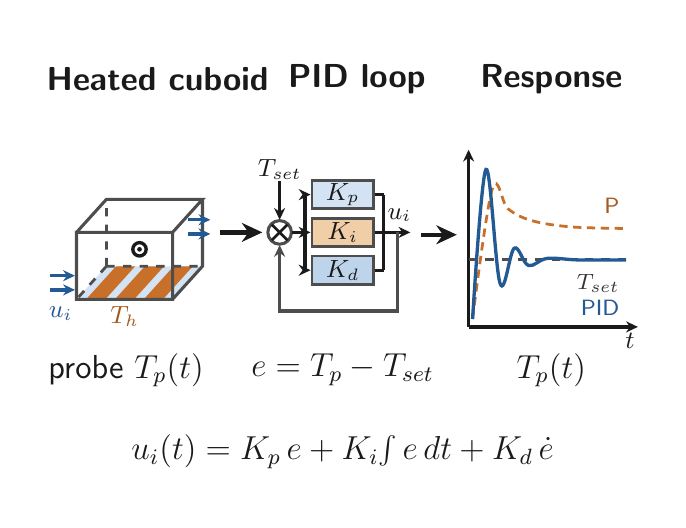
\begin{tikzpicture}[
    line width=1.6pt, >={Stealth[length=2.6mm,width=2.4mm]},
    small arrow/.style={-{Stealth[length=1.5mm,width=1.4mm]}, line width=1.2pt},
    color=ink,
    title/.style={font=\large\bfseries, text=ink},
    lab/.style={font=\large, text=ink},
    gain/.style={draw=frame, line width=1.0pt, minimum width=0.78cm, minimum height=0.36cm,
                 inner sep=0pt, font=\small, text=ink}]
  % fixed 8 cm x 6 cm canvas
  \path[use as bounding box] (0,0) rectangle (8,6);

  % ================= 1) heated cuboid with inlet, outlet and probe =================
  \node[title] at (1.65,5.35) {Heated cuboid};
  \def\xo{0.62} \def\yo{2.55} \def\w{1.22} \def\h{0.85} \def\dx{0.38} \def\dy{0.42}
  % bottom plane with three discrete heated strips (T_h)
  \fill[mist] (\xo,\yo) -- ++(\w,0) -- ++(\dx,\dy) -- ++(-\w,0) -- cycle;
  \foreach \a in {0.10,0.40,0.70}
    \fill[amber] (\xo+\a*\w,\yo) -- ++(0.2*\w,0) -- ++(\dx,\dy) -- ++(-0.2*\w,0) -- cycle;
  % hidden back edges
  \draw[frame, line width=1.0pt, dashed] (\xo+\dx,\yo+\dy) -- ++(\w,0)
        (\xo+\dx,\yo+\dy) -- ++(0,\h) (\xo+\dx,\yo+\dy) -- ++(-\dx,-\dy);
  % visible edges
  \draw[frame, line width=1.1pt]
        (\xo,\yo) rectangle ++(\w,\h)
        (\xo,\yo+\h) -- ++(\dx,\dy) -- ++(\w,0) -- ++(-\dx,-\dy)
        (\xo+\w+\dx,\yo+\h+\dy) -- ++(0,-\h) -- ++(-\dx,-\dy);
  % inlet (cool air, lower left) and outlet (upper right)
  \foreach \y in {0.12,0.30}
    \draw[small arrow, steel] (\xo-0.34,\yo+\y) -- (\xo-0.02,\yo+\y);
  \foreach \y in {0.62,0.80}
    \draw[small arrow, steel] (\xo+\w+0.20,\yo+\y+0.21) -- (\xo+\w+0.48,\yo+\y+0.21);
  % temperature probe at the centre
  \fill[white] (\xo+0.5*\w+0.19,\yo+0.5*\h+0.21) circle (0.085);
  \draw[ink, line width=1.2pt] (\xo+0.5*\w+0.19,\yo+0.5*\h+0.21) circle (0.085);
  \fill[ink] (\xo+0.5*\w+0.19,\yo+0.5*\h+0.21) circle (0.03);
  \node[font=\small, text=steel] at (\xo-0.20,\yo-0.18) {$u_i$};
  \node[font=\small, text=amber!80!black] at (\xo+0.5*\w,\yo-0.22) {$T_h$};
  \node[lab] at (1.25,1.65) {probe $T_p(t)$};

  % ================= 2) PID feedback loop =================
  \node[title] at (4.18,5.35) {PID loop};
  % summing junction e = T_p - T_set
  \draw[frame, line width=1.1pt, fill=white] (3.20,3.40) circle (0.15);
  \draw[ink, line width=1.0pt] (3.20,3.40) ++(-0.10,-0.10) -- ++(0.20,0.20) ++(-0.20,0) -- ++(0.20,-0.20);
  \node[font=\small] at (3.20,4.20) {$T_{set}$};
  \draw[small arrow] (3.20,4.05) -- (3.20,3.56);
  % three gains
  \node[gain, fill=mist] (kp) at (4.00,3.88) {$K_p$};
  \node[gain, fill=sand] (ki) at (4.00,3.40) {$K_i$};
  \node[gain, fill=sky!45] (kd) at (4.00,2.92) {$K_d$};
  \draw[line width=1.2pt] (3.36,3.40) -- (3.52,3.40);
  \draw[line width=1.2pt] (3.52,3.88) -- (3.52,2.92);
  \foreach \n in {kp,ki,kd} \draw[small arrow] (3.52,0 |- \n.west) -- (\n.west);
  \foreach \n in {kp,ki,kd} \draw[line width=1.2pt] (\n.east) -- (4.52,0 |- \n.east);
  \draw[line width=1.2pt] (4.52,3.88) -- (4.52,2.92);
  \draw[small arrow] (4.52,3.40) -- (4.86,3.40);
  \node[font=\small] at (4.72,3.62) {$u_i$};
  % feedback path
  \draw[small arrow, frame] (4.70,3.40) -- (4.70,2.40) -- (3.20,2.40) -- (3.20,3.24);
  \node[lab] at (4.00,1.65) {$e = T_p - T_{set}$};

  % ================= 3) temperature response =================
  \node[title] at (6.65,5.35) {Response};
  \draw[small arrow] (5.60,2.20) -- (7.75,2.20);
  \draw[small arrow] (5.60,2.20) -- (5.60,4.45);
  \node[font=\small] at (7.65,2.02) {$t$};
  % set point
  \draw[frame, line width=1.1pt, dashed] (5.60,3.05) -- (7.65,3.05);
  \node[font=\footnotesize, anchor=north east, text=frame!70!black] at (7.66,3.01) {$T_{set}$};
  % P: settles with a steady-state error
  \draw[amber, line width=1.0pt, dash pattern=on 3pt off 2pt]
    plot[smooth, tension=0.6] coordinates
      {(5.65,2.30) (5.90,3.95) (6.10,3.70) (6.40,3.55) (6.90,3.47) (7.60,3.45)};
  % PID: overshoot, then settles on the set point
  \draw[steel, line width=1.2pt]
    plot[smooth, tension=0.6] coordinates
      {(5.65,2.30) (5.82,4.20) (6.00,2.75) (6.18,3.20) (6.36,2.98) (6.60,3.07) (7.00,3.05) (7.60,3.05)};
  \node[font=\footnotesize, text=amber!80!black, anchor=south east] at (7.66,3.50) {P};
  \node[font=\footnotesize, text=steel, anchor=north east] at (7.66,2.68) {PID};
  \node[lab] at (6.65,1.65) {$T_p(t)$};

  % ================= arrows between panels =================
  \draw[->] (2.44,3.40) -- (2.98,3.40);
  \draw[->] (5.00,3.37) -- (5.45,3.37);

  % ================= control law =================
  \node[font=\large, text=ink] at (4.00,0.62)
    {$u_i(t) = K_p\,e + K_i\!\int e\,dt + K_d\,\dot e$};
\end{tikzpicture}
\end{document}
